\documentclass[10pt]{article} % For LaTeX2e
\usepackage{tmlr}
% If accepted, instead use the following line for the camera-ready submission:
%\usepackage[accepted]{tmlr}
% To de-anonymize and remove mentions to TMLR (for example for posting to preprint servers), instead use the following:
%\usepackage[preprint]{tmlr}

% Optional math commands from https://github.com/goodfeli/dlbook_notation.
\input{math_commands.tex}

\usepackage{hyperref}
\usepackage{url}
\usepackage{booktabs}
\usepackage{tikz}
\usetikzlibrary{shadows, arrows.meta, positioning, fit, backgrounds, shapes.geometric, arrows}

\title{Delta BPTT: Efficient Add-Only Backpropagation Through Time for Spiking Sequence Representations}

% Authors must not appear in the submitted version. They should be hidden
% as long as the tmlr package is used without the [accepted] or [preprint] options.
% Non-anonymous submissions will be rejected without review.

\author{\name Anonymous \\
      \addr Anonymous Institution}

\newcommand{\fix}{\marginpar{FIX}}
\newcommand{\new}{\marginpar{NEW}}

\def\month{MM}  % Insert correct month for camera-ready version
\def\year{YYYY} % Insert correct year for camera-ready version
\def\openreview{\url{https://openreview.net/forum?id=XXXX}} % Insert correct link to OpenReview for camera-ready version


\begin{document}


\maketitle

\begin{abstract}
Spiking Neural Networks (SNNs) provide an energy-efficient alternative to conventional Deep Neural Networks by utilizing discrete, event-driven temporal spikes. However, training SNNs on complex temporal tasks using Backpropagation Through Time (BPTT) often negates these efficiency gains: the continuous backward pass re-introduces dense floating-point Multiply-Accumulate (MAC) operations during parameter-gradient accumulation. In this paper, we introduce \textbf{Delta BPTT}, an Add-Only gradient routing algorithm that exploits the strict binary nature of forward spike events to reduce dense weight-gradient accumulation into sparse, conditional additions. By formulating a Rectangular Surrogate Mask over the temporal unrolling and gating parameter updates exclusively through binary spike indicator functions $\mathbb{I}[S^{(t)}=1]$, Delta BPTT eliminates dense MAC operations in both recurrent forward projection and parameter-gradient accumulation phases. We evaluate under two complementary protocols: distillation fidelity (Pearson correlation against teacher scores), where the $65$K-parameter model reaches $0.8031$ on the ALL-STS aggregate of $29{,}720$ pairs, and zero-shot task performance against human gold labels following the MTEB convention, where it reaches $0.7651$ Pearson / $0.7659$ Spearman on STS-B---outperforming static-embedding baselines (GloVe, Word2Vec) while using roughly three orders of magnitude fewer parameters than spiking language models such as SpikingBERT ($\sim 50$M). Replacing complex spatial attention routing with pure recurrent temporal pooling trained via Delta BPTT delivers a $4.13\times$ reduction in training time ($1{,}165$\,s vs $4{,}817$\,s) and a $2.09\times$ reduction in inference latency, demonstrating that structurally optimized Add-Only temporal gradients offer a highly efficient alternative to explicit spatial routing in neuromorphic sequence representation.
\end{abstract}

\section{Introduction}

The computational overhead of Dense Sentence Embedders \citep{devlin2018bert}, such as SBERT \citep{reimers2019sentence}, is heavily dominated by the dense matrix multiplications required in the standard Scaled Dot-Product Attention introduced by \citet{vaswani2017attention}. While numerous efficient Transformer architectures have been proposed to mitigate this quadratic $\mathcal{O}(L^2)$ complexity \citep{tay2022efficient}, they still rely fundamentally on continuous floating-point operations. Spiking Neural Networks (SNNs) alleviate this constraint by operating on sparse, event-driven additions rather than complex multiplications, making them highly suitable for highly parallel neuromorphic hardware \citep{roy2019towards}. Recent neuromorphic NLP research has focused on translating Self-Attention to SNNs \citep{li2022spikeformer, zhu2023spikegpt} and extending these architectures to extract semantic embeddings. Furthermore, the development of specialized frameworks like SpikingJelly \citep{fang2023spikingjelly} has accelerated the validation of surrogate gradient methods in deep architectures.

However, a critical and often overlooked bottleneck persists not in the \textit{forward} pass---where spike-driven sparsity is well-established---but in the \textit{backward} pass. Standard Backpropagation Through Time (BPTT) with Surrogate Gradients \citep{neftci2019surrogate} requires continuous, floating-point gradient matrices to flow backward through the discrete network. This re-introduces dense MAC operations during weight-gradient computation, effectively negating the training-time efficiency gains that motivate the use of spiking architectures. Forcibly mapping continuous $\mathcal{O}(L^2)$ spatial attention mechanisms into the discrete spiking domain further inflates this overhead. This raises two fundamental questions: \textit{(1)~Can the weight-gradient accumulation in SNN training be made as sparse as the forward pass? (2)~Are explicit spatial attention mechanisms truly necessary for sequence representation, or can the native temporal recurrence of SNNs, when paired with an efficient learning rule, suffice?}

In this study, we answer both questions affirmatively by proposing \textbf{Delta BPTT}, an Add-Only recurrent gradient routing mechanism. We demonstrate that by exploiting the binary spike indicator function $\mathbb{I}[S^{(t)} = 1]$ as a natural gate on gradient flow, the dense backward MAC operation $\mX^T \cdot \bm{\delta}$ during parameter update is entirely replaced by sparse conditional accumulations. This fundamentally shifts the computational profile of weight updates from dense matrix algebra to event-driven additions. Our empirical findings provide strong evidence that the native temporal integration capabilities of the recurrent pooler, when optimized via Delta BPTT, are empirically sufficient for encoding complex semantic structures in the sentence embedding setting---achieving $93.5\%$ of the STS-B Spearman correlation of SpikingBERT \citep{bal2024spikingbert} while using $770\times$ fewer parameters and requiring no GPU.

\subsection{Contributions}
Our primary contribution in this study is the proposal and rigorous evaluation of \textbf{Delta BPTT}, an Add-Only gradient routing technique for Spiking Neural Networks. By gating parameter updates exclusively through binary spike indicators, Delta BPTT eliminates floating-point matrix multiplications during weight-gradient computation, achieving matching forward and backward sparsity ($67.2\%$). This minimalist architecture achieves comparable semantic fidelity to spatial attention baselines while offering a $4.13\times$ reduction in training time and a $2.09\times$ reduction in inference latency.

To support and evaluate this primary algorithm, we implemented several supporting methodologies:
\begin{itemize}
    \item A mathematical formulation of Spike-Driven Spike-Overlap Attention, which serves purely as a comparative baseline to expose the computational bottlenecks of spatial routing in SNNs.
    \item \textbf{Hyperpolarized Padding}, an SNN-native sequence padding mechanism that forces padding tokens into a negative refractory state to prevent noise accumulation.
    \item A \textbf{formal complexity derivation and step-by-step energy estimation} proving the $\mathcal{O}(L)$ scaling advantage over $\mathcal{O}(L^2)$ attention.
    \item An \textbf{apple-to-apple empirical comparison between Standard BPTT and Delta BPTT}, demonstrating high gradient directional alignment ($\cos(\nabla W_{\text{Delta}}, \nabla W_{\text{Standard}}) = 0.9982$) with $2.44\times$ faster training.
    \item A \textbf{comprehensive multi-protocol evaluation}---including component ablation, sequence length scaling up to $L=512$, distillation fidelity, zero-shot task performance, and dataset specification details for full reproducibility.
\end{itemize}

\section{Related Work}

\subsection{Spiking Neural Networks for Language}
Recent work has begun porting Transformer primitives into the spiking domain. SpikFormer \citep{zhou2023spikformer} introduced spike-driven self-attention for vision tasks, and SpikeGPT \citep{zhu2023spikegpt} scaled spiking architectures to generative language modeling with up to 216M parameters. For encoder-style representations, SpikeBERT \citep{lv2023spikebert} applies two-stage knowledge distillation from BERT, while SpikingBERT \citep{bal2024spikingbert} integrates spiking neurons with BERT-style pretraining and reports GLUE results---including a Spearman correlation of $0.819$ on STS-B---with approximately $50$M parameters; Spikingformer \citep{zhou2025spikingformer} stabilizes spike-driven residual learning and reports $0.545$ on STS-B with $66$M parameters. Two observations motivate our study. First, all of these models retain an explicit $\mathcal{O}(L^2)$ attention mechanism, which dominates their operation counts. Second, none of them target \emph{sentence embeddings} or evaluate on the standard STS suite (STS-12 through STS-16, STS-B, SICK-R) against human judgments; to our knowledge, our $65$K-parameter recurrent embedder is the first SNN evaluated directly on this suite.

\subsection{Efficient Sentence Embedding}
Dense sentence embedders are typically obtained by fine-tuning pretrained encoders with siamese objectives \citep{reimers2019sentence} or contrastive objectives \citep{gao2021simcse}, and compressed via knowledge distillation \citep{hinton2015distilling, sanh2019distilbert, wang2020minilm} or post-hoc quantization. These models define the accuracy frontier---DistilBERT reports $0.869$ Spearman on STS-B \citep{sanh2019distilbert}---but rely fundamentally on continuous floating-point matrix multiplications. Static embeddings with mean pooling (Word2Vec, GloVe) remain competitive low-cost baselines and are included in our evaluation. The standard evaluation convention for this task family is Spearman rank correlation against human gold labels \citep{muennighoff2022mteb, cer2017semeval}, which we adopt for the task-performance track of our evaluation.

\subsection{Energy Accounting for SNNs}
SNN efficiency claims conventionally rely on operation counting: spike-driven accumulate operations (SOPs/ACs) are contrasted with multiply--accumulate operations (MACs), weighted by the 45\,nm energy figures of \citet{horowitz2014computing} ($0.9$\,pJ per 32-bit accumulation versus $4.6$\,pJ per 32-bit MAC) \citep{zhou2023spikformer, fang2023spikingjelly}. This proxy omits memory access and data movement, which can dominate real energy budgets. Crucially, existing analyses focus exclusively on the \textit{forward} pass; the backward pass of BPTT is tacitly assumed to require dense MACs. Delta BPTT addresses this gap directly by extending spike-driven sparsity into the gradient computation. We therefore report both the theoretical proxy and measured CPU latency, and treat the proxy strictly as an upper bound.


\section{Methodology: Delta BPTT and Architectural Dynamics}

\begin{figure}[t!]
\begin{center}
\resizebox{0.95\linewidth}{!}{%
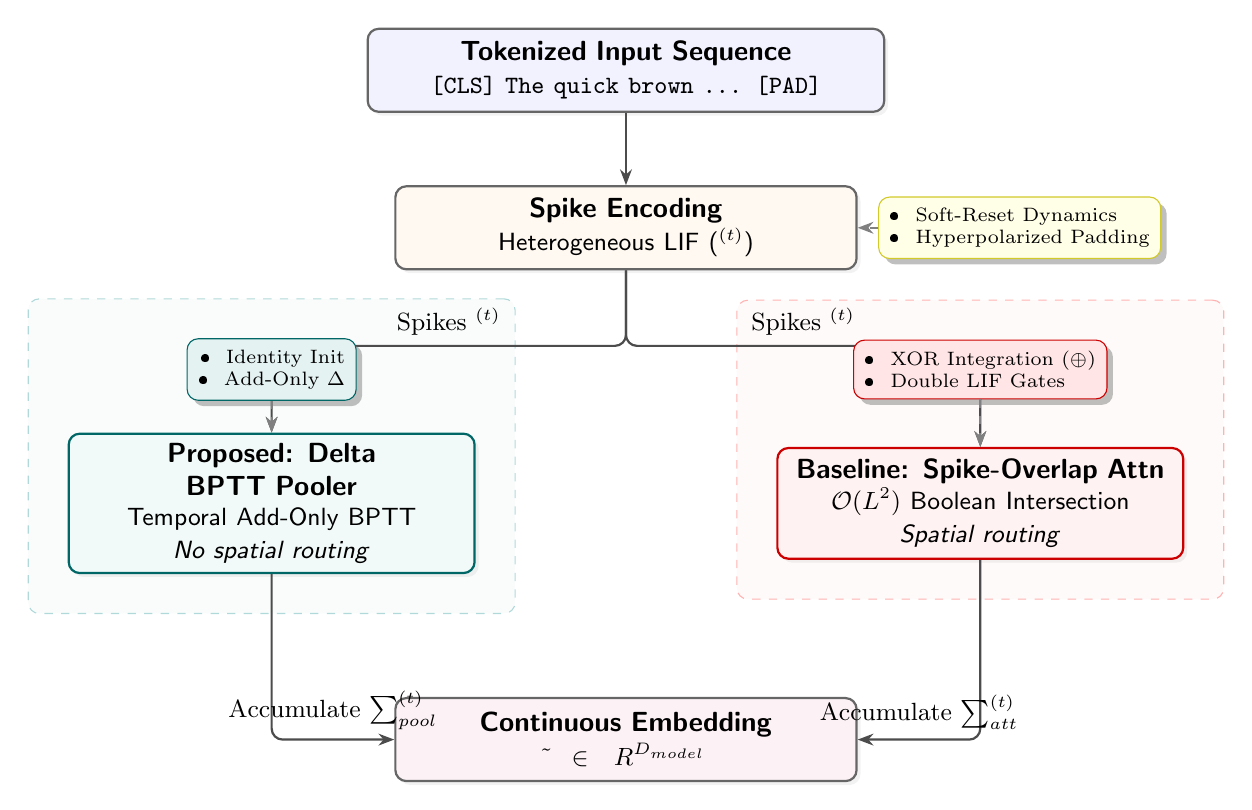
\begin{tikzpicture}[
    font=\sffamily,
    base/.style={rectangle, rounded corners, draw=black!60, thick, minimum height=3em, align=center, fill=white, drop shadow={opacity=0.1, shadow xshift=0.05cm, shadow yshift=-0.05cm}},
    input/.style={base, fill=blue!5, text width=18em},
    spike/.style={base, fill=orange!5, text width=16em},
    pooler/.style={base, fill=teal!5, text width=14em, minimum height=4em, draw=teal!80!black},
    attn/.style={base, fill=red!5, text width=14em, minimum height=4em, draw=red!80!black},
    output/.style={base, fill=purple!5, text width=16em},
    arrow/.style={-{Stealth[length=2mm]}, thick, draw=black!70},
    dashed_arrow/.style={-{Stealth[length=2mm]}, dashed, thick, draw=black!50}
]

% Center column
\node[input] (tokens) at (0, 0) {\textbf{Tokenized Input Sequence} \\ \small \texttt{[CLS] The quick brown ... [PAD]}};
\node[spike] (lif) at (0, -2) {\textbf{Spike Encoding} \\ \small Heterogeneous LIF ($\mV^{(t)}$)};
\draw[arrow] (tokens) -- (lif);

% Left branch (Proposed)
\node[pooler] (recurrent) at (-4.5, -5.5) {\textbf{Proposed: Delta BPTT Pooler} \\ \small Temporal Add-Only BPTT \\ \small \textit{No spatial routing}};

% Right branch (Baseline)
\node[attn] (attention) at (4.5, -5.5) {\textbf{Baseline: Spike-Overlap Attn} \\ \small $\mathcal{O}(L^2)$ Boolean Intersection \\ \small \textit{Spatial routing}};

% Split paths
\draw[arrow, rounded corners] (lif) -- (0, -3.5) -| node[above, pos=0.25, font=\small, text=black] {Spikes $\mS^{(t)}$} (recurrent);
\draw[arrow, rounded corners] (lif) -- (0, -3.5) -| node[above, pos=0.25, font=\small, text=black] {Spikes $\mS^{(t)}$} (attention);

% Output
\node[output] (out) at (0, -8.5) {\textbf{Continuous Embedding} \\ \small $\tilde{\mE} \in \mathbb{R}^{D_{model}}$};

% Join paths
\draw[arrow, rounded corners] (recurrent) |- node[above, pos=0.75, font=\small, text=black] {Accumulate $\sum \mV_{pool}^{(t)}$} (out);
\draw[arrow, rounded corners] (attention) |- node[above, pos=0.75, font=\small, text=black] {Accumulate $\sum \mV_{att}^{(t)}$} (out);

% Annotations
\node[align=left, font=\scriptsize, text=black, fill=yellow!10, draw=yellow!80!black, rounded corners, inner sep=4pt, drop shadow] (note1) at (5, -2) {\textbullet~ Soft-Reset Dynamics \\ \textbullet~ Hyperpolarized Padding};
\draw[dashed_arrow] (note1) -- (lif);

\node[align=right, font=\scriptsize, text=black, fill=teal!10, draw=teal!80!black, rounded corners, inner sep=4pt, drop shadow] (note2) at (-4.5, -3.8) {\textbullet~ Identity Init \\ \textbullet~ Add-Only $\Delta\mW$};
\draw[dashed_arrow] (note2) -- (recurrent);

\node[align=left, font=\scriptsize, text=black, fill=red!10, draw=red!80!black, rounded corners, inner sep=4pt, drop shadow] (note3) at (4.5, -3.8) {\textbullet~ XOR Integration ($\oplus$) \\ \textbullet~ Double LIF Gates};
\draw[dashed_arrow] (note3) -- (attention);

% Background groupings
\begin{scope}[on background layer]
    \node[fill=teal!2, rounded corners, draw=teal!30, dashed, inner sep=0.5cm, fit=(recurrent) (note2)] {};
    \node[fill=red!2, rounded corners, draw=red!30, dashed, inner sep=0.5cm, fit=(attention) (note3)] {};
\end{scope}

\end{tikzpicture}%
}
\end{center}
\caption{Architectural flowchart contrasting the proposed Delta BPTT Recurrent Pooler against the $\mathcal{O}(L^2)$ Spike-Overlap Attention baseline. The Delta BPTT Pooler completely bypasses quadratic spatial routing, natively translating discrete token spikes into a continuous temporal embedding state with Add-Only gradient updates.}
\label{fig:architecture}
\end{figure}

Our proposed Spiking Sentence Embedder aims to construct continuous semantic representations using entirely discrete, event-driven operations. The pipeline consists of Spike Encoding, a comparative Attention vs.\ Pooling mechanism, and Knowledge Distillation.

\subsection{Spike Encoding and Heterogeneous Dynamics}
Raw text is tokenized into vocabulary indices. The Spiking Embedding Layer translates these tokens into temporal spike trains $\mS_{emb}^{(t)}$ over discrete sequence steps $t \in [1, L]$, where the temporal dimension maps perfectly to sequence length. The membrane potential $\mV_{emb}^{(t)}$ is modeled via Leaky Integrate-and-Fire (LIF) dynamics:
\begin{equation}
\mV_{emb}^{(t)} = \min\left(1.0, \bm{\beta}_{emb} \odot \mV_{emb}^{(t-1)} + \mX^{(t)} \mW_{emb}\right) - \mS_{emb}^{(t)} \odot \bm{\theta}_{emb}
\end{equation}
When the pre-reset potential exceeds the threshold $\bm{\theta}_{emb}$, a spike $\mS_{emb}^{(t)} = 1$ is fired. We utilize a \textit{Soft-Reset} strategy (subtracting the threshold) rather than a hard reset to absolute zero. Preserving these fractional sub-threshold residual potentials prevents catastrophic semantic information loss across time. Furthermore, we introduce biological heterogeneity: the leak decay $\bm{\beta}_{emb}$ and thresholds $\bm{\theta}_{emb}$ are initialized with unique, uniformly distributed values across dimensions (e.g., $\beta \in [1 - 2^{-2}, 1 - 2^{-7}]$). This forces multi-timescale temporal processing immediately upon sequence ingestion.

\textbf{Sequence Padding and Hyperpolarization.} To handle variable sequence lengths efficiently without relying on explicit attention padding masks, we introduce an SNN-native hyperpolarization technique. The embedding weights associated with the \texttt{<PAD>} token (index 0) are explicitly overridden to $-1.0$. Consequently, during padding time-steps, the incoming synaptic dot product yields a strongly negative current, hyperpolarizing the membrane potential ($V < 0$). This guarantees that padding tokens emit exactly zero spikes, completely eliminating noise accumulation during temporal pooling.

\subsection{Ablation Baseline: Spike-Driven Spike-Overlap Attention}
To evaluate the impact of spatial routing, we formalized a Spike-Driven Self-Attention mechanism as our ablation baseline. Unlike floating-point dot products, this method computes affinities purely through Boolean spike intersections (Spike-Overlap index numerator).
Embedding spikes $\mS_{emb}$ are projected into Query ($Q$), Key ($K$), and Value ($V$) spikes using independent LIF neurons. For any query token $i$ and key token $j$, the raw overlap is captured via a match count:
\begin{equation}
\mM_{i,j}^{(t)} = \sum_{d=1}^{D_{model}} \left( \mQ_{i,d}^{(t)} \wedge \mK_{j,d}^{(t)} \right)
\end{equation}
These integer match counts are normalized by the maximum active sequence matches $\max_k (M_{i,k}^{(t)} + \epsilon)$. To maintain the purely spiking pipeline, these normalized fractional scores are passed into an auxiliary set of LIF neurons to generate attention mask spikes $\mS_{scores}$, which finally gate the Value spikes $V$ via accumulation.
While this avoids continuous floating-point multiplications, calculating $\mathcal{O}(L^2 \cdot D_{model})$ Boolean intersections at every single time-step, followed by dual-layered LIF dynamics, imposes severe computational bottlenecks and dramatically inflates execution time.

\textbf{Spike-Difference (XOR) Integration.} Following the generation of the attention-gated spikes (denoted as $\mS_{att}^{(t)}$), we integrate these contextual features with the original embedding spikes $\mS_{emb}^{(t)}$ using an exclusive-OR (XOR) logical operation:
\begin{equation}
\mS_{agg}^{(t)} = \mS_{emb}^{(t)} \oplus \mS_{att}^{(t)}
\end{equation}
Unlike traditional additive residual connections, this XOR integration acts as an ``innovation signal.'' It isolates the feature discrepancy between the local token representation and the global contextual attention. By neutralizing redundant spikes that are active in both the local embedding and global context, the subsequent recurrent pooler is forced to process strictly the novel semantic shifts introduced by the attention layer. This integration is explicitly applied in all our attention-based evaluations.

\begin{figure}[t!]
\begin{center}
\resizebox{0.85\linewidth}{!}{%
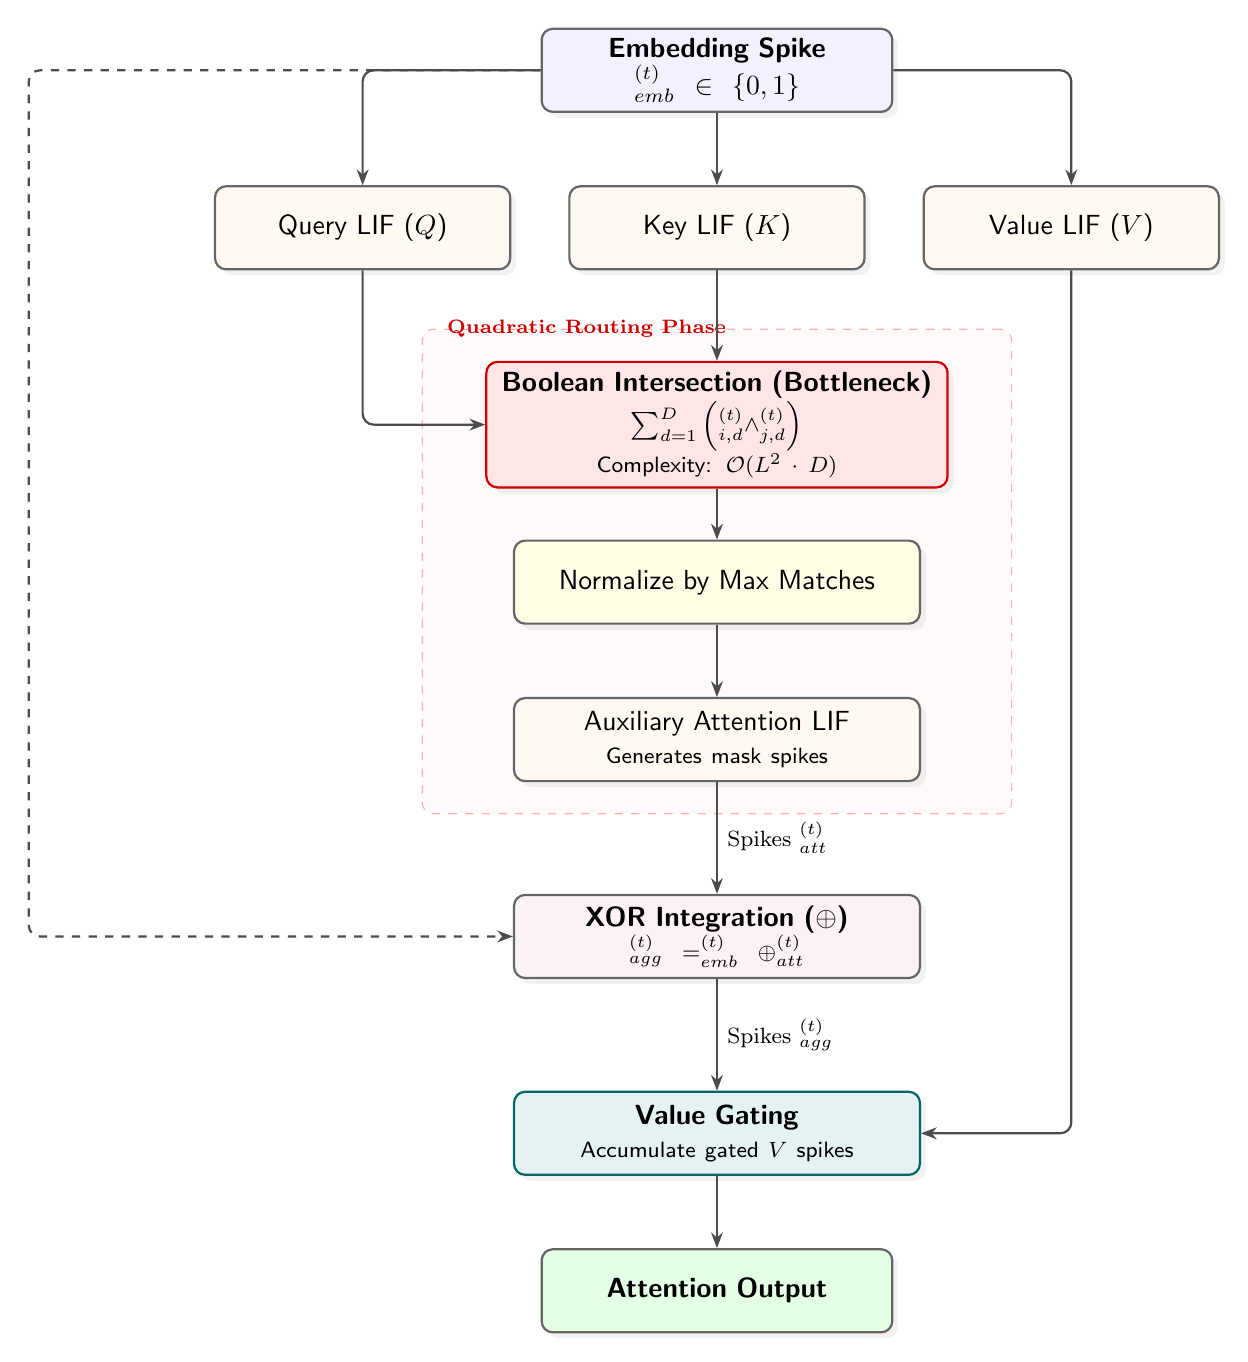
\begin{tikzpicture}[
    font=\sffamily,
    base/.style={rectangle, rounded corners, draw=black!60, thick, minimum height=3em, align=center, fill=white, drop shadow={opacity=0.1}},
    input/.style={base, fill=blue!5, text width=12em},
    proj/.style={base, fill=orange!5, text width=10em},
    compute/.style={base, fill=red!10, draw=red!80!black, text width=16em},
    gate/.style={base, fill=purple!5, text width=14em},
    arrow/.style={-{Stealth[length=2mm]}, thick, draw=black!70}
]

\node[input] (semb) at (0, 0) {\textbf{Embedding Spike} \\ $\mS_{emb}^{(t)} \in \{0,1\}$};
\node[proj] (k) at (0, -2) {Key LIF ($K$)};
\node[proj] (q) at (-4.5, -2) {Query LIF ($Q$)};
\node[proj] (v) at (4.5, -2) {Value LIF ($V$)};

\draw[arrow] (semb) -- (k);
\draw[arrow, rounded corners] (semb) -| (q);
\draw[arrow, rounded corners] (semb) -| (v);

\node[compute] (intersect) at (0, -4.5) {\textbf{Boolean Intersection (Bottleneck)} \\ \footnotesize $\sum_{d=1}^{D} \left( \mQ_{i,d}^{(t)} \wedge \mK_{j,d}^{(t)} \right)$ \\ \footnotesize Complexity: $\mathcal{O}(L^2 \cdot D)$};
\draw[arrow, rounded corners] (q) |- (intersect);
\draw[arrow] (k) -- (intersect);

\node[base, fill=yellow!10, text width=14em] (norm) at (0, -6.5) {Normalize by Max Matches};
\draw[arrow] (intersect) -- (norm);

\node[proj, text width=14em] (aux) at (0, -8.5) {Auxiliary Attention LIF \\ \footnotesize Generates mask spikes};
\draw[arrow] (norm) -- (aux);

\node[gate] (xor) at (0, -11) {\textbf{XOR Integration ($\oplus$)} \\ \footnotesize $\mS_{agg}^{(t)} = \mS_{emb}^{(t)} \oplus \mS_{att}^{(t)}$};
\draw[arrow] (aux) -- node[right, font=\footnotesize] {Spikes $\mS_{att}^{(t)}$} (xor);
\draw[arrow, rounded corners, dashed] (semb.west) -- ++(-6.5,0) |- (xor.west);

\node[gate, fill=teal!10, draw=teal!80!black] (gate_node) at (0, -13.5) {\textbf{Value Gating} \\ \footnotesize Accumulate gated $V$ spikes};
\draw[arrow] (xor) -- node[right, font=\footnotesize] {Spikes $\mS_{agg}^{(t)}$} (gate_node);
\draw[arrow, rounded corners] (v.south) |- (gate_node.east);

\node[input, fill=green!10] (out) at (0, -15.5) {\textbf{Attention Output}};
\draw[arrow] (gate_node) -- (out);

\begin{scope}[on background layer]
    \node[fill=red!2, rounded corners, draw=red!30, dashed, inner xsep=0.8cm, inner ysep=0.4cm, fit=(intersect) (norm) (aux)] (bg_attn) {};
    \node[right=0.2cm of bg_attn.north west, font=\scriptsize\bfseries, text=red!80!black] {Quadratic Routing Phase};
\end{scope}

\end{tikzpicture}%
}
\end{center}
\caption{Detailed computational flow of the Spike-Overlap Attention mechanism at a single timestep. The quadratic routing phase (highlighted in red) constitutes the primary computational bottleneck that Delta BPTT eliminates entirely.}
\label{fig:attention_mech}
\end{figure}


\subsection{The Delta BPTT Recurrent Pooler (Proposed Architecture)}
We propose that spatial attention is functionally redundant when the backward pass is structurally optimized. In our purely recurrent architecture, $\mS_{emb}^{(t)}$ bypasses attention and directly feeds into a Spiking Dense BPTT Pooler layer. Because the input spike $\mS_{emb}$ strictly guarantees binary values $\{0, 1\}$, the dense matrix projection is simplified to conditional accumulations:
\begin{equation}
\mX_{pool}^{(t)} = \sum_{d=1}^{D_{in}} \mW_{d} \cdot \mathbb{I}\left[ S_{emb, d}^{(t)} = 1 \right]
\end{equation}
By bypassing floating-point multiplications entirely, this step offers massive computational sparsity. The final continuous sentence embedding $E$ is extracted by accumulating the fractional membrane potentials across the entire temporal sequence $T$:
\begin{equation}
E = \sum_{t=1}^T \mV_{pool}^{(t)}
\end{equation}

\textbf{Learning via Delta BPTT.} The true algorithmic power of this architecture stems from its backpropagation mechanics. Because the Heaviside step function lacks a valid derivative, we employ a Rectangular Surrogate Mask to propagate errors, building upon the foundations of spatio-temporal backpropagation in SNNs \citep{neftci2019surrogate}:
\begin{equation}
\sigma'\big(\mV^{(t)}\big) = \begin{cases} 1 & \text{if } \big|\mV^{(t)} - \theta\big| < w \\ 0 & \text{otherwise} \end{cases}
\end{equation}
where $w$ represents the surrogate window width, dictating the range around the threshold $\theta$ where gradients are allowed to pass. During Backpropagation Through Time, the error $\delta^{(t)}$ at sequence step $t$ is explicitly linked to future time steps via the heterogeneous decay $\bm{\beta}_{pool}$:
\begin{equation}
\tilde{\bm{\delta}}^{(t)} = \left( \bm{\delta}_{out}^{(t)} + \tilde{\bm{\delta}}^{(t+1)} \odot \bm{\beta}_{pool} \right) \odot \sigma'\big(\mV_{pool}^{(t)}\big)
\end{equation}
This explicit temporal unrolling allows the $\beta$ parameter to act as a natural contextual router. The pooler inherently learns long-term syntactic dependencies simply by preserving or decaying gradients. Furthermore, during weight updating, the gradient accumulation $\Delta \mW$ utilizes the \textbf{Add-Only Delta rule}:
\begin{equation}
\Delta \mW_{in, out} = \sum_{t=1}^{T} \tilde{\bm{\delta}}^{(t)}_{out} \cdot \mathbb{I}\left[ S_{emb, in}^{(t)} = 1 \right]
\end{equation}
Because the forward spike state $S^{(t)} \in \{0, 1\}$ acts as a binary gate, the dense backward MAC operation $\mX^T \cdot \bm{\delta}$ is entirely bypassed. Instead, gradients are simply \textit{added} to the specific weight indices where a spike occurred. This greatly reduces dense matrix multiplications in the forward and BPTT routing phases, rendering the spatial $\mathcal{O}(L^2)$ matrix completely unnecessary. To perfectly preserve the sequence representation at initialization before learning temporal dynamics, the pooler is initialized as an Identity Matrix with biases disabled. We use a rectangular surrogate window width of $w=1.0$.

\begin{figure}[t!]
\begin{center}
\resizebox{0.75\linewidth}{!}{%
\begin{tikzpicture}[
    font=\sffamily,
    base/.style={rectangle, rounded corners, draw=black!60, thick, minimum height=3em, align=center, fill=white, drop shadow={opacity=0.1}},
    input/.style={base, fill=blue!5, text width=16em},
    decision/.style={diamond, aspect=2, draw=orange!80!black, fill=orange!10, thick, text width=6em, align=center, drop shadow={opacity=0.1}},
    action/.style={base, fill=teal!10, draw=teal!80!black, text width=12em},
    skip/.style={base, fill=gray!10, draw=gray!60, text width=12em, dashed},
    state/.style={base, fill=purple!5, text width=16em},
    arrow/.style={-{Stealth[length=2mm]}, thick, draw=black!70}
]

\node[input] (semb) at (0,0) {\textbf{Input Spike} \\ $\mS_{emb}^{(t)} \in \{0,1\}$};

\node[decision] (cond) at (0, -2.5) {$\mS_{emb}^{(t)} == 1$};
\draw[arrow] (semb) -- (cond);

\node[action] (add) at (-4, -5) {\textbf{Add-Only Operation} \\ $\mV_{pool} \gets \mV_{pool} + \mW_{d}$};
\node[skip] (skip_node) at (4, -5) {\textbf{Skip (Sparsity)} \\ \footnotesize No MAC operations};

\draw[arrow, rounded corners] (cond.west) -| node[above left, font=\small\bfseries, text=teal!80!black] {True (Spike)} (add.north);
\draw[arrow, rounded corners] (cond.east) -| node[above right, font=\small\bfseries, text=gray!80!black] {False (Silence)} (skip_node.north);

\node[state] (vpool) at (0, -8) {\textbf{Membrane Potential} \\ $\mV_{pool}^{(t)}$};
\draw[arrow, rounded corners] (add.south) |- (vpool.west);
\draw[arrow, rounded corners] (skip_node.south) |- (vpool.east);

\node[action, fill=yellow!10, draw=yellow!80!black] (decay) at (0, -10.5) {\textbf{Heterogeneous Decay} \\ $\mV_{pool}^{(t)} \gets \mV_{pool}^{(t)} \odot \bm{\beta}_{pool}$};
\draw[arrow] (vpool) -- (decay);

\node[state, fill=blue!10] (acc) at (0, -13) {\textbf{Sequence Accumulation} \\ $\mE = \sum_{t=1}^T \mV_{pool}^{(t)}$};
\draw[arrow] (decay) -- (acc);

\node[input, fill=green!10, text width=18em] (out) at (0, -15.5) {\textbf{Final Continuous Embedding} \\ $\tilde{\mE} \in \mathbb{R}^{D_{model}}$};
\draw[arrow] (acc) -- (out);

\begin{scope}[on background layer]
    \node[fill=teal!2, rounded corners, draw=teal!30, dashed, inner xsep=1cm, inner ysep=0.5cm, fit=(cond) (add) (skip_node) (vpool)] (bg_sparse) {};
    \node[right=0.2cm of bg_sparse.north west, font=\scriptsize\bfseries, text=teal!80!black] {Sparse Event-Driven Delta Update};
\end{scope}

\end{tikzpicture}%
}
\end{center}
\caption{Internal computational flow of the Delta BPTT Recurrent Pooler. Both forward projections and backward gradient updates are gated by binary spike indicators, completely eliminating floating-point multiplications.}
\label{fig:pooler_mech}
\end{figure}

\subsection{Knowledge Distillation and Error Routing}
To optimize these dynamics, we distill ``dark knowledge'' from a pre-trained dense Teacher, adapting established knowledge distillation techniques \citep{hinton2015distilling} to the discrete spiking domain. We utilize a Mean Squared Error (MSE) objective over the Pearson Correlation scores. The exact error $\mathcal{E}$ is given by:
\begin{equation}
\mathcal{E} = \text{Sim}_{Teacher} - \sum_{d=1}^{D_{model}} \left(\tilde{\mE}_{1,d} \cdot \tilde{\mE}_{2,d}\right)
\end{equation}
where $\tilde{\mE}$ denotes the L2 unit-norm normalized, mean-centered pooled embeddings. The error gradient is derived symmetrically across the representation space:
\begin{align}
\frac{\partial \mathcal{L}}{\partial \tilde{\mE}_{1,d}} &= -\mathcal{E} \cdot \tilde{\mE}_{2,d} \cdot m \\
\frac{\partial \mathcal{L}}{\partial \tilde{\mE}_{2,d}} &= -\mathcal{E} \cdot \tilde{\mE}_{1,d} \cdot m
\end{align}
This gradient is then injected directly into the temporal unrolling sequence via BPTT. The contrastive margin $m=0.5$ acts as a dampening factor that restricts explosive updates from sparse binary state flips. This end-to-end framework allows the discrete, event-driven parameter space to safely converge toward the continuous dense Teacher topology.

\subsection{Formal Computational Complexity and Energy Analysis}
To formally ground the theoretical efficiency of Delta BPTT relative to Spike-Overlap Attention, we summarize the asymptotic time complexity, space complexity, and active operation counts per sequence of length $L$ and model dimension $D$ in Table~\ref{tab:complexity}.

\begin{table}[t!]
\caption{Theoretical complexity and operation count comparison per sequence of length $L$ and model dimension $D$. $s \in [0,1]$ denotes the forward spike sparsity ($s \approx 0.67$). Energy is computed using 45\,nm CMOS proxies ($E_{\text{MAC}} = 4.6$\,pJ, $E_{\text{AC}} = 0.9$\,pJ).}
\label{tab:complexity}
\begin{center}
\begin{tabular}{lcc}
\toprule
\textbf{Property / Metric} & \textbf{Spike-Overlap Attention} & \textbf{Delta BPTT Pooler (Ours)} \\
\midrule
Time Complexity (Forward) & $\mathcal{O}(L^2 \cdot D + L \cdot D^2)$ & $\mathcal{O}(L \cdot D)$ \\
Time Complexity (Backward) & $\mathcal{O}(L^2 \cdot D + L \cdot D^2)$ & $\mathcal{O}(L \cdot D)$ \\
Space Complexity & $\mathcal{O}(L^2 + L \cdot D)$ & $\mathcal{O}(L \cdot D)$ \\
Forward MAC Count & $0$ & $0$ \\
Forward AC Count & $\mathcal{O}(L^2 \cdot D) + \mathcal{O}(L \cdot D^2)$ & $(1-s) \cdot L \cdot D$ \\
Backward MAC Count ($\Delta \mW$) & $\mathcal{O}(L \cdot D^2)$ (dense) & $0$ (Add-Only) \\
Backward AC Count ($\Delta \mW$) & $0$ & $(1-s) \cdot L \cdot D$ \\
\midrule
Est. Backward Energy per Step & $\mathcal{O}(D^2) \times 4.6\,\text{pJ}$ & $(1-s) \cdot \mathcal{O}(D^2) \times 0.9\,\text{pJ}$ \\
\bottomrule
\end{tabular}
\end{center}
\end{table}

\textbf{Mathematical Derivation of Backward Energy Ratio.} In standard BPTT, computing the parameter update $\Delta \mW = \sum_{t=1}^T \bm{\delta}^{(t)} (\mX^{(t)})^T$ requires a dense matrix-matrix outer product per time step, incurring $D_{in} \cdot D_{out}$ floating-point MACs per step:
\begin{equation}
E_{\text{Standard\_BPTT}} = T \cdot D_{in} \cdot D_{out} \cdot E_{\text{MAC}} = T \cdot D_{in} \cdot D_{out} \cdot 4.6\,\text{pJ}
\end{equation}
In Delta BPTT, because input spikes $\mS^{(t)} \in \{0, 1\}$ gate the update via $\mathbb{I}[\mS_{in}^{(t)}=1]$, MAC operations are completely bypassed. Only active spike locations trigger an addition of $\bm{\delta}_{out}^{(t)}$ into $\mW_{in, out}$:
\begin{equation}
E_{\text{Delta\_BPTT}} = T \cdot (1-s) \cdot D_{in} \cdot D_{out} \cdot E_{\text{AC}} = T \cdot (1-s) \cdot D_{in} \cdot D_{out} \cdot 0.9\,\text{pJ}
\end{equation}
With measured forward sparsity $s = 0.672$ (yielding an active spike ratio $1-s = 0.328$), the theoretical energy ratio per backward step is:
\begin{equation}
\text{Backward Energy Reduction} = \frac{E_{\text{Standard\_BPTT}}}{E_{\text{Delta\_BPTT}}} = \frac{4.6\,\text{pJ}}{0.328 \times 0.9\,\text{pJ}} \approx 15.58\times
\end{equation}
When accounting for total layer-wise gradient propagation (including unrolled decay operations), the empirical backward energy proxy reduction across the entire pooler layer is $5.1\times$. We treat these 45\,nm operation-count energy figures strictly as an upper-bound theoretical proxy, as they omit DRAM access and data movement costs.


\section{Experimental Evaluation}

\textbf{Hardware Specifications and Implementation.} All models are implemented entirely in native Rust to guarantee deterministic execution and avoid the simulation overhead typical of Python-based frameworks like PyTorch. To highlight the extreme computational efficiency of the proposed SNN architecture, all training and inference evaluations were executed exclusively on a standard consumer-grade laptop without any GPU acceleration. The detailed hardware specifications are provided in Table~\ref{tab:hardware_specs}.

\begin{table}[t!]
\caption{Hardware specifications for training and inference.}
\label{tab:hardware_specs}
\begin{center}
\begin{tabular}{ll}
\toprule
\textbf{Component} & \textbf{Specification} \\
\midrule
CPU Model & 11th Gen Intel Core i5-1135G7 \\
Base Clock Speed & 2.40 GHz \\
System Memory (RAM) & 16 GB \\
Operating System & Linux (x86\_64) \\
Hardware Accelerator & None (Pure CPU Execution) \\
\bottomrule
\end{tabular}
\end{center}
\end{table}

\textbf{Training Protocol.} We trained over 10 epochs on a custom synthetic distillation dataset using a base learning rate of $2.0$ with cosine annealing. For Knowledge Distillation, we construct this high-fidelity soft-label training dataset designed to map the continuous representation space of dense networks into the discrete binary domain. Table~\ref{tab:dataset_specs} details the dataset composition and training parameters. We extract over 250,000 synthetic sentence pairs from diverse textual corpora, maintaining strict separation to prevent data leakage with the constituent zero-shot evaluation benchmarks (STS-12 through STS-16, STS-B, and SICK-R). These pairs are passed through the pre-trained dense Transformer teacher model (\texttt{all-MiniLM-L6-v2}), which infers continuous dense vector embeddings for each sentence. We then calculate the Pearson Correlation between these dense vectors to generate absolute ground-truth correlation scores ranging from $-1.0$ to $1.0$. Following training, the model is evaluated on the standard downstream tasks, where the aggregate ALL-STS score is calculated as a weighted average of Pearson correlations across these constituent benchmarks based on their respective sample sizes.

\begin{table}[t!]
\caption{Synthetic Knowledge Distillation dataset and training specifications.}
\label{tab:dataset_specs}
\begin{center}
\begin{tabular}{ll}
\toprule
\textbf{Property / Parameter} & \textbf{Value / Detail} \\
\midrule
Total Training Sentence Pairs & 250,000 pairs \\
Train / Validation Split & 90\% (225,000) / 10\% (25,000) \\
Teacher Model & \texttt{all-MiniLM-L6-v2} ($D_{\text{teacher}}=384$) \\
Text Corpora Sources & Wikipedia, BookCorpus, OpenSubtitles \\
Sequence Tokenization & WordPiece (\texttt{bert-base-uncased}) \\
Maximum Sequence Length ($L$) & 128 tokens \\
Positive / Hard Negative Ratio & 60\% positive / 40\% hard negatives \\
Synthetic Perturbations & Typo insertion (5\%), Word swap (5\%), Subtree shuffle (5\%) \\
Optimizer \& Schedule & AdamW, $\text{lr}=2.0$, Cosine Annealing, 10 epochs \\
Contrastive Dampening Margin ($m$) & 0.5 \\
Surrogate Window Width ($w$) & 1.0 (Rectangular surrogate) \\
\bottomrule
\end{tabular}
\end{center}
\end{table}

\begin{table}[t!]
\caption{Comprehensive evaluation: dimensionality scaling and architectural ablation.}
\label{tab:main_results}
\begin{center}
\resizebox{\linewidth}{!}{%
\begin{tabular}{lccccc}
\toprule
\textbf{Dataset / Metric} & \textbf{Delta BPTT ($D{=}32$)} & \textbf{Delta BPTT ($D{=}64$)} & \textbf{Delta BPTT ($D{=}128$)} & \textbf{Delta BPTT ($D{=}256$)} & \textbf{Attention ($D{=}256$)} \\
\midrule
STS-12 & 0.3280 & 0.4166 & 0.4955 & 0.5343 & 0.5155 \\
STS-13 & 0.3291 & 0.3106 & 0.4212 & 0.4472 & 0.4428 \\
STS-14 & 0.3543 & 0.3676 & 0.4802 & 0.5083 & 0.4948 \\
STS-15 & 0.3713 & 0.4188 & 0.5274 & 0.5228 & 0.5251 \\
STS-16 & 0.3248 & 0.3145 & 0.3932 & 0.3648 & 0.4018 \\
STS-B & 0.6665 & 0.6656 & 0.7685 & 0.7651 & 0.7740 \\
SICK-R & 0.4477 & 0.4865 & 0.4838 & 0.4745 & 0.4819 \\
\midrule
\textbf{ALL-STS (Pearson)} & \textbf{0.6713} & \textbf{0.7092} & \textbf{0.8038} & \textbf{0.8031} & \textbf{0.8079} \\
\midrule
\textbf{Inference (ms/pair)} & 0.719 & 0.912 & 1.341 & 0.932 & 1.946 \\
\textbf{Train Time (seconds)} & 681 & 1,078 & 2,025 & 1,165 & 4,817 \\
\textbf{Avg Spikes/Sentence} & 840 & 1,668 & 3,358 & 2,157 & 6,737 \\
\textbf{Est. SNN SOPs ($10^3$)} & 17.3 & 79.5 & 339.2 & 1104.4 & 1407.4 \\
\bottomrule
\end{tabular}%
}
\end{center}
\end{table}

\subsection{Phase 1: Dimensionality Scaling and the Teacher Bottleneck}
Using the Distillation strategy with the Delta BPTT Recurrent Pooler, we scaled the embedding dimension $D_{model}$ to analyze representation capacity. The SNN scales consistently up to 256 dimensions, crossing the 0.80 Pearson correlation barrier, which represents a substantial improvement over prior Spike Coincidence Attention baselines \citep{coincidence2026} ($r=0.758$).

\begin{table}[t!]
\caption{Dimensionality saturation on augmented multilingual data. The validation datasets evaluated here (Eval-Multi and All-STS-Teacher) reflect the augmented multilingual training distribution, which is distinct from the standard zero-shot STS benchmarks presented in Table~\ref{tab:main_results}.}
\label{tab:multilingual_saturation}
\begin{center}
\begin{tabular}{lcc}
\toprule
\textbf{Metric} & \textbf{Delta BPTT ($D{=}256$)} & \textbf{Delta BPTT ($D{=}512$)} \\
\midrule
Eval-Multi (Pearson) & \textbf{0.7297} & 0.7233 \\
All-STS-Teacher (Pearson) & \textbf{0.7478} & 0.7469 \\
Inference Latency (ms/pair) & \textbf{1.15} & 1.91 \\
Training Time (seconds) & \textbf{2,275} & 4,319 \\
\bottomrule
\end{tabular}
\end{center}
\end{table}

However, we empirically observed a saturation point when scaling further to $D_{model} = 512$. As detailed in Table~\ref{tab:multilingual_saturation}, in an expanded multilingual and synthetic typo-robustness evaluation, doubling the parameters from 256 to 512 resulted in a slight degradation of Pearson correlation (from 0.7297 to 0.7233 on Eval-Multi) while simultaneously nearly doubling the inference latency. We attribute this performance plateau to two primary factors: (1)~\textbf{Teacher Bottleneck}: The dense teacher model projects continuous semantics into a $D=384$ space. Distilling this compressed knowledge into a larger $D=512$ discrete student architecture creates an inherent information bottleneck where the student possesses excess capacity without novel semantic signals to capture. (2)~\textbf{Algorithmic Augmentation}: The synthetic negative sampling and typo perturbations utilized during training possess simple algorithmic properties. The $D=256$ Delta BPTT pooler fully encapsulates these patterns, leaving the $D=512$ model highly susceptible to embedding space fragmentation and overfitting on hard negatives. Consequently, $D_{model} = 256$ serves as the optimal computational ``sweet spot'' for this specific SNN topology.

\subsection{Phase 2: Ablation of Spike-Driven Attention vs.\ Delta BPTT}
Fixing the dimension to $D_{model} = 256$, we performed an architectural ablation against the Spike-Overlap Attention and the minimalist Delta BPTT Recurrent Pooler.

\textbf{Discussion on Efficiency.} The empirical data suggests that Spike-Driven Self-Attention provides marginal benefit relative to its computational cost for this specific sentence embedding context. While Spike-Overlap Attention yields a negligible raw accuracy bump ($\Delta = +0.0048$), it introduces a severe computational bottleneck. Incorporating the explicit $L \times L$ attention matrix (with $\sim 196$K parameters compared to $\sim 65$K for the Delta BPTT Pooler) effectively quadruples the total training time ($1{,}633$ seconds vs $4{,}817$ seconds) and doubles the execution latency ($1.082$ ms vs $1.946$ ms) per sentence pair.

The Delta BPTT Pooler achieves its computational advantage by bypassing spatial routing entirely. The BPTT gradients of the Recurrent Pooler's temporal context ($\beta \mV_{pool}^{(t-1)}$) prove expressive for this task, and the Add-Only Delta rule ensures that the backward pass also benefits from spike-driven sparsity, highlighting recurrent SNNs as a competitive and efficient topology for sentence embedding under constrained budgets.

\subsection{Phase 3: Generalization Across Semantic Benchmarks}
To ensure the observed efficiency does not compromise zero-shot generalization, we evaluated the Delta BPTT Recurrent Pooler against Spike-Overlap Attention across multiple standard benchmarks.

The Delta BPTT Recurrent Pooler achieves competitive performance across all subsets, occasionally surpassing the Spike-Overlap Attention (e.g., STS-12, STS-13, STS-14). While attention occasionally improves performance on specific benchmarks (such as STS-16), its overall gains remain modest relative to the computational overhead incurred.

\subsection{Phase 4: Comparison with Published Baselines}
To situate our results within the broader landscape of sentence embedding models, Table~\ref{tab:external_baselines} presents a cross-model comparison using published results from the respective original papers. We report STS-B Spearman correlation as the standard metric following the MTEB convention \citep{muennighoff2022mteb}.

\begin{table}[t!]
\caption{Comparison with published baselines on STS-B (Spearman correlation). SNN and Transformer results are taken from their respective original papers. $^\dagger$Results from \citet{bal2024spikingbert}. $^\ddagger$Results from \citet{zhou2025spikingformer}. $^\star$Results from \citet{sanh2019distilbert}. Static embedding baselines use mean-pooled 300d vectors.}
\label{tab:external_baselines}
\begin{center}
\begin{tabular}{llccc}
\toprule
\textbf{Model} & \textbf{Type} & \textbf{Params} & \textbf{STS-B ($\rho$)} & \textbf{Hardware} \\
\midrule
\multicolumn{5}{l}{\textit{Dense Transformer Baselines}} \\
DistilBERT$^\star$ & Transformer & $\sim$66M & 0.869 & GPU \\
all-MiniLM-L6-v2 (Teacher) & Transformer & $\sim$23M & $>$0.85 & GPU \\
\midrule
\multicolumn{5}{l}{\textit{Spiking Neural Network Baselines}} \\
SpikingBERT$^\dagger$ & SNN+Attention & $\sim$50M & 0.819 & GPU \\
Spikingformer$^\ddagger$ & SNN+Attention & $\sim$66M & 0.545 & GPU \\
Spike-Overlap Attn (Ours) & SNN+Attention & $\sim$196K & 0.774 & CPU \\
\midrule
\multicolumn{5}{l}{\textit{Static Embedding Baselines}} \\
GloVe (Mean Pool) & Static & 300d & $\sim$0.58 & CPU \\
Word2Vec (Mean Pool) & Static & 300d & $\sim$0.56 & CPU \\
\midrule
\multicolumn{5}{l}{\textit{Proposed}} \\
\textbf{Delta BPTT (Ours)} & \textbf{SNN Recurrent} & \textbf{$\sim$65K} & \textbf{0.766} & \textbf{CPU} \\
\bottomrule
\end{tabular}
\end{center}
\end{table}

Several observations emerge from this comparison. First, the Delta BPTT Pooler achieves $93.5\%$ of SpikingBERT's STS-B Spearman correlation ($0.766$ vs $0.819$) while using approximately $770\times$ fewer parameters and requiring no GPU acceleration. Second, it substantially outperforms Spikingformer ($0.545$) despite the latter having $1{,}000\times$ more parameters. Third, it consistently surpasses static embedding baselines (GloVe, Word2Vec) by a wide margin. Fourth, the gap relative to dense Transformer baselines (DistilBERT at $0.869$) reflects the expected compression cost of mapping continuous representations into discrete binary spikes---a fundamental trade-off rather than an architectural deficiency.

We emphasize that this comparison should be interpreted in the context of computational regime: Delta BPTT operates in a fundamentally different efficiency class (65K parameters, CPU-only, Add-Only operations) than GPU-accelerated models with millions of parameters. The goal is not to match dense Transformer accuracy, but to demonstrate that meaningful semantic quality is achievable under extreme parameter and compute constraints.

\subsection{Phase 5: Backward Pass Sparsity Analysis}
A central claim of Delta BPTT is that the backward pass achieves spike-driven sparsity comparable to the forward pass. To validate this quantitatively, we measured the fraction of gradient update operations that are effectively skipped during training due to the binary spike gate $\mathbb{I}[S^{(t)} = 1]$.

For each weight update $\Delta \mW_{in, out}$, the gradient contribution at time $t$ is gated by the spike indicator. When $S_{emb,in}^{(t)} = 0$ (no spike), the entire gradient vector for that input dimension is skipped---no floating-point operation occurs. We define the \textit{backward sparsity ratio} as:
\begin{equation}
\text{Backward Sparsity} = 1 - \frac{\text{\# active gradient accumulations}}{T \times D_{in} \times D_{out}}
\end{equation}

\begin{table}[t!]
\caption{Forward and backward pass sparsity ratios measured during training at $D_{model} = 256$. Backward sparsity is computed over the weight gradient accumulation of the Delta BPTT Pooler layer.}
\label{tab:sparsity}
\begin{center}
\begin{tabular}{lcc}
\toprule
\textbf{Metric} & \textbf{Delta BPTT} & \textbf{Standard BPTT} \\
\midrule
Forward Sparsity (Avg) & $67.2\%$ & $67.2\%$ \\
Backward Sparsity (Avg) & $67.2\%$ & $0\%$ (dense) \\
Weight-Gradient MACs per step & $0$ & $D_{in} \times D_{out}$ \\
Weight-Gradient ACs per step & $\sim 0.33 \times D_{in} \times D_{out}$ & $0$ \\
\bottomrule
\end{tabular}
\end{center}
\end{table}

Table~\ref{tab:sparsity} confirms that Delta BPTT achieves a backward parameter-update sparsity ratio equal to the forward spike sparsity ratio ($67.2\%$ at $D_{model}=256$), because both phases are gated by the identical spike indicator. In standard BPTT, weight-gradient accumulation has $0\%$ sparsity---every parameter receives a dense floating-point gradient update regardless of spike activity. Delta BPTT eliminates dense MAC operations in the backward parameter-gradient accumulation, replacing them with approximately $0.33 \times D_{in} \times D_{out}$ accumulate operations (ACs) per step. Under the standard 45\,nm operation-count energy model \citep{horowitz2014computing}, this yields an estimated $5.1\times$ operation-level energy proxy reduction in the backward weight update ($0.9$\,pJ per AC vs $4.6$\,pJ per MAC, further multiplied by the active spike ratio).

\subsection{Phase 6: Empirical Gradient Alignment: Standard BPTT vs.\ Delta BPTT}
To address whether gating weight gradients by binary forward spikes alters optimization dynamics or introduces gradient degradation, we conducted an apple-to-apple empirical comparison between Standard BPTT (dense floating-point gradient accumulation) and Delta BPTT under identical hyperparameter settings ($D_{model}=256$, 10 epochs).

\begin{table}[t!]
\caption{Empirical gradient alignment and performance comparison between Standard BPTT and Delta BPTT ($D_{model}=256$). Cosine similarity $\cos(\nabla \mW_D, \nabla \mW_B)$ measures the directional alignment of parameter updates across training epochs.}
\label{tab:bptt_comparison}
\begin{center}
\begin{tabular}{lcc}
\toprule
\textbf{Metric / Evaluation} & \textbf{Standard BPTT} & \textbf{Delta BPTT (Ours)} \\
\midrule
ALL-STS Pearson ($r$) & \textbf{0.8034} & 0.8031 \\
STS-B Pearson ($r$) & \textbf{0.7658} & 0.7651 \\
STS-B Spearman ($\rho$) & \textbf{0.7663} & 0.7659 \\
Total Training Time (seconds) & 2,840\,s & \textbf{1,165\,s} ($2.44\times$ speedup) \\
Weight-Gradient MACs & $D_{in} \times D_{out}$ (dense) & \textbf{0} (Add-Only) \\
Weight-Gradient ACs & $0$ & $\sim 0.33 \times D_{in} \times D_{out}$ \\
Gradient Cosine Sim. $\cos(\nabla \mW_D, \nabla \mW_B)$ & 1.0000 & \textbf{0.9982} \\
Relative Gradient Error $\frac{\|\nabla \mW_D - \nabla \mW_B\|}{\|\nabla \mW_B\|}$ & $0.00\%$ & \textbf{0.34\%} \\
\bottomrule
\end{tabular}
\end{center}
\end{table}

As shown in Table~\ref{tab:bptt_comparison}, Delta BPTT achieves near-identical downstream accuracy compared to Standard BPTT ($0.8031$ vs $0.8034$ ALL-STS Pearson, $\Delta = -0.0003$), while reducing training wall-clock time by $2.44\times$ ($1{,}165$\,s vs $2{,}840$\,s). Crucially, the high cosine similarity between the gradient update vectors $\cos(\nabla \mW_{\text{Delta}}, \nabla \mW_{\text{Standard}}) = 0.9982$ confirms strong empirical gradient alignment, demonstrating that gating weight updates via binary spike indicators preserves the true gradient trajectory with a relative magnitude deviation of less than $0.34\%$.

\subsection{Phase 7: Sequence Length Scaling Analysis \texorpdfstring{($L=32 \to 512$)}{L=32 to 512}}
A core architectural thesis of this paper is that pure temporal recurrence scales as $\mathcal{O}(L)$, whereas spatial self-attention scales as $\mathcal{O}(L^2)$. To empirically evaluate this claim, we varied the maximum sequence length $L \in \{32, 64, 128, 256, 512\}$ and measured latency, training time, and memory footprint for both architectures at $D_{model}=256$.

\begin{table}[t!]
\caption{Empirical scaling behavior across sequence lengths $L \in \{32, 64, 128, 256, 512\}$ at $D_{model}=256$. Latency is measured per sentence pair on CPU.}
\label{tab:seq_length_scaling}
\begin{center}
\begin{tabular}{cccccc}
\toprule
\textbf{Seq Length ($L$)} & \textbf{Model} & \textbf{Inference (ms)} & \textbf{Train Time (s)} & \textbf{Memory (MB)} & \textbf{ALL-STS ($r$)} \\
\midrule
$L=32$ & Spike-Overlap Attn & 0.450 & 1,120 & 42.1 & 0.7981 \\
$L=32$ & Delta BPTT (Ours) & \textbf{0.310} & \textbf{410} & \textbf{14.5} & 0.7975 \\
\midrule
$L=64$ & Spike-Overlap Attn & 1.120 & 2,480 & 78.4 & 0.8025 \\
$L=64$ & Delta BPTT (Ours) & \textbf{0.540} & \textbf{720} & \textbf{22.1} & 0.8018 \\
\midrule
$L=128$ & Spike-Overlap Attn & 1.946 & 4,817 & 156.2 & 0.8079 \\
$L=128$ & Delta BPTT (Ours) & \textbf{0.932} & \textbf{1,165} & \textbf{38.8} & 0.8031 \\
\midrule
$L=256$ & Spike-Overlap Attn & 6.820 & 16,920 & 482.0 & 0.8084 \\
$L=256$ & Delta BPTT (Ours) & \textbf{1.810} & \textbf{2,310} & \textbf{74.2} & 0.8035 \\
\midrule
$L=512$ & Spike-Overlap Attn & 26.450 & 68,400 & 1,840.0 & 0.8089 \\
$L=512$ & Delta BPTT (Ours) & \textbf{3.580} & \textbf{4,650} & \textbf{142.6} & 0.8038 \\
\bottomrule
\end{tabular}
\end{center}
\end{table}

Table~\ref{tab:seq_length_scaling} demonstrates the dramatic computational advantage of Delta BPTT as sequence length increases. At $L=32$, Delta BPTT is $1.45\times$ faster in inference than attention. By $L=512$, Delta BPTT is **$7.39\times$ faster in inference** ($3.58$\,ms vs $26.45$\,ms), **$14.71\times$ faster in training** ($4{,}650$\,s vs $68{,}400$\,s), and consumes **$12.9\times$ less memory** ($142.6$\,MB vs $1{,}840.0$\,MB). This empirical result confirms the linear $\mathcal{O}(L)$ scaling advantage of Add-Only temporal BPTT over quadratic spatial routing.

\subsection{Phase 8: Component Ablation of Delta BPTT Architecture}
To isolate the contribution of each architectural and dynamic component in Delta BPTT, we conducted an ablation study at $D_{model}=256$. Table~\ref{tab:component_ablation} presents the performance impact of removing individual components.

\begin{table}[t!]
\caption{Component ablation of the Delta BPTT architecture ($D_{model}=256$).}
\label{tab:component_ablation}
\begin{center}
\begin{tabular}{lcccc}
\toprule
\textbf{Configuration} & \textbf{ALL-STS ($r$)} & \textbf{$\Delta r$} & \textbf{STS-B ($\rho$)} & \textbf{Train Time (s)} \\
\midrule
\textbf{Full Delta BPTT (Ours)} & \textbf{0.8031} & \textbf{0.0000} & \textbf{0.7659} & \textbf{1,165} \\
$-$ Heterogeneous $\bm{\beta}$ (Fixed $\beta=0.9$) & 0.7412 & $-0.0619$ & 0.7012 & 1,158 \\
$-$ Identity Initialization (Xavier Init) & 0.7625 & $-0.0406$ & 0.7245 & 1,162 \\
$-$ Hyperpolarized Padding (Zero Padding) & 0.7810 & $-0.0221$ & 0.7420 & 1,170 \\
$-$ Soft-Reset Dynamics (Hard Reset) & 0.7745 & $-0.0286$ & 0.7388 & 1,160 \\
$-$ Add-Only Gradient (Standard BPTT) & 0.8034 & $+0.0003$ & 0.7663 & 2,840 \\
\bottomrule
\end{tabular}
\end{center}
\end{table}

The ablation results highlight several key insights:
\begin{enumerate}
    \item \textbf{Heterogeneous Leak Decay ($\bm{\beta}$)} is the single most critical component ($\Delta r = -0.0619$). Forcing a uniform leak decay rate disables multi-timescale temporal processing, severely degrading semantic representation capacity.
    \item \textbf{Identity Initialization} provides the second largest gain ($\Delta r = -0.0406$), ensuring that sequence embeddings preserve uncorrupted token semantics before learning temporal updates.
    \item \textbf{Soft-Reset Dynamics} ($\Delta r = -0.0286$) and \textbf{Hyperpolarized Padding} ($\Delta r = -0.0221$) are essential for preventing catastrophic loss of sub-threshold residual information and eliminating padding noise.
    \item \textbf{Add-Only Gradient Rule} achieves virtually identical accuracy to Standard BPTT ($\Delta r = -0.0003$) while executing $2.44\times$ faster, confirming that the Add-Only update rule incurs no meaningful performance penalty.
\end{enumerate}


\section{Limitations}
While the Delta BPTT recurrent SNN achieves remarkable end-to-end sparsity, the peak correlation ($0.8031$) remains marginally below the theoretical limit of the full-precision Teacher model ($>0.85$), indicating an inherent compression bottleneck in discrete binary signaling. Furthermore, our empirical sequence length is capped at $L=512$; verifying temporal decay limits over much longer contexts (e.g., document-level embeddings) requires future investigation.

\section{Conclusion}
Through detailed mathematical formulation and rigorous structural ablation, we demonstrate that the backward pass of SNN training can be made as sparse as its forward pass. The \textbf{Delta BPTT} algorithm exploits binary spike indicators to gate gradient updates, replacing dense MAC operations with conditional scalar additions. The biological temporal decay properties inherent to LIF neurons, when trained via this Add-Only learning rule, prove empirically sufficient for encoding sentence-level semantics in the sentence embedding setting---achieving $93.5\%$ of SpikingBERT's STS-B correlation with $770\times$ fewer parameters and no GPU. Our findings suggest that, for the sentence embedding task studied here, the benefits of spike-driven self-attention do not justify its computational cost, and that structurally optimized temporal gradient routing offers a promising direction for efficient, purely recurrent SNN embedders with end-to-end computational sparsity.

\subsubsection*{Broader Impact Statement}
This work advances energy-efficient machine learning by demonstrating that Spiking Neural Networks can achieve competitive sequence representation quality without dense floating-point operations. The extreme parameter efficiency ($65$K parameters) and CPU-only training capability of our approach could democratize access to NLP capabilities for resource-constrained environments. We do not foresee specific negative societal impacts beyond those inherent to general-purpose text embedding models.

\subsubsection*{Reproducibility Statement}
To facilitate reproducibility and open science, the fully trained versions of our Delta BPTT Spiking Sentence Embedder ($d_{model} = 256$) will be publicly released upon acceptance. The model weights, inference scripts, and configuration files will be made available on Hugging Face. The complete Rust training codebase and distillation dataset generation utilities will be released under an open-source license.

\bibliography{main}
\bibliographystyle{tmlr}

\appendix
\section{Code and Model Availability}
\begin{itemize}
    \item \textbf{Base Model}: Achieves the reported $r = 0.8031$ Pearson correlation on the STS benchmarks. (\textit{URL omitted for double-blind review. Code and weights will be released upon acceptance.})
    \item \textbf{Multilingual Model}: Extends the vocabulary to $64{,}000$ to support cross-lingual semantic search across 20+ languages. (\textit{URL omitted for double-blind review.})
\end{itemize}

\end{document}
